\input{../.preambles/01-semester_work}
\input{../.preambles/10-russian}
\input{../.preambles/20-math}
\input{../.preambles/30-physics}
\usepackage{wrapfig}

\begin{document}
\maketitlepage{Факультет электроники и вычислительной техники}{физики}
{Квантовая теория}{}{6}{студент группы Ф-369\\Голубев~А.~В.}
{}{доцент Жуков~С.~С.}{}{}

%-------------------------------------------------------------------------------

\emph{Задача №1:} Вычислить длину волны де Бройля для тепловых 
(\( T = 300 \) K) нейтронов. Следует ли учитывать волновые свойства нейтронов 
при анализе их взаимодействия с кристаллом? Расстояние между атомами в 
кристалле принять равным 0,50 нм.

\emph{Решение:}

Рассмотрим нерелятивистский случай \( v_\text{тепл.} \ll c \).

Длина волны де Бройля выражается формулой: \( \lambda = \cfrac{h}{p} \)

Импульс теплового нейтрона можно выразить из формулы: 
\[	
	E = \frac{p^2}{2m}
\] 

где \( E = kT \), \( m \) -- масса покоя нейтрона.

Подставляя в формулу для длины волны получим:
\[
	\lambda = \frac{h}{\sqrt{2mkT}} = 
	\frac{6.63\cdot10^{-34}}
	{\sqrt{2\cdot300\cdot1.67\cdot10^{-27}\cdot1.38\cdot10^{-23}}} =
	178 \text{ пм}
\]

Воспользуемся принципом неопределённости Гейзенберга:
\[
	\Delta x \cdot \Delta p_x \geq \frac{\hbar}{2}
\]

Положим \( l \sim \Delta x \), \( p \sim \Delta p_x \). Тогда получаем:
\[
	l\cdot \sqrt{2mkT} \geq \frac{\hbar}{2} 
\]

или
\[ 
	0.5\cdot10^{-9} \cdot 
	\sqrt{2\cdot300\cdot1.67\cdot10^{-27}\cdot1.38\cdot10^{-23}} \geq
	\frac{1.06\cdot10^{-34}}{2}
\]

и сравнивая полученные величины по их порядкам
\[
	10^{-24} \geq 10^{-34}
\]

Отсюда следует, что при взаимодействии с кристаллом можно не учитывать волновые 
свойства нейтронов.

\pagebreak
%-------------------------------------------------------------------------------

\emph{Задача №2:} Частица массы \( m \) движется в одномерной прямоугольной 
потенциальной яме с бесконечно высокими стенками. Ширина ямы \( l \). Найти 
значения энергии частицы, имея в виду, что возможны лишь такие состояния, для 
которых в яме укладывается целое число дебройлевских полуволн. 

\emph{Решение:}

Запишем однородное уравнение Шрёдингера для частицы в 
прямоугольной потенциальной яме с бесконечно высокими стенками.
\[
	-\frac{\hbar^2}{2m}\dder{\psi(x)}{x} = E\psi(x)
\] 
\[
	\dder{\psi(x)}{x}+\frac{2mE}{\hbar^2}\psi(x) = 0
\]

Обозначим производную по координате штрихами:
\[
	\psi''(x) + k^2 \psi(x) = 0
\]

Представим решение в виде функции 
\( \psi(x) = A\sin\left( kx + \alpha \right) \). Применим 
граничные условия:
\[
	\psi(0) = \psi(l) = 0; \quad
\]
\[
	\psi(0) = A\sin\alpha = 0 \Rightarrow \alpha = 0
\]
\[
	\psi(l) = A\sin\left( kl \right) = 0 \Rightarrow kl = \pi n, 
	\text{ где } n = 1, 2, 3, ...; \quad k = \frac{\pi n}{l}
\]

Найдём первую и вторую производные:
\[
	\psi' = A\frac{\pi n}{l}\cos\left( \frac{\pi nx}{l} \right);\quad
	\psi'' = -A\left(\frac{\pi n}{l} \right)^2 
		\sin\left( \frac{\pi nx}{l} \right)
\]

и подставляя полученные функции в уравнение Шрёдингера, получим:
\[
	\frac{2mE}{\hbar^2} = \left( \frac{\pi n}{l} \right)^2
\]

Откуда получаем значения энергии частицы:
\[
	E_n = \frac{1}{2m}\left( \frac{n\pi\hbar}{l} \right)^2
\]

\pagebreak
%-------------------------------------------------------------------------------

\emph{Задача №3:} Частица массы \( m \) падает на прямоугольный потенциальный 
барьер \( U(x) = \alpha\delta(x) \). Энергия частицы \( E \). Найти коэффициент 
прозрачности \( D \) и коэффициент прохождения \( R \) барьера.

\emph{Решение:}

\begin{wrapfigure}[10]{l}{0.5\textwidth}
    \vspace{-2ex}
    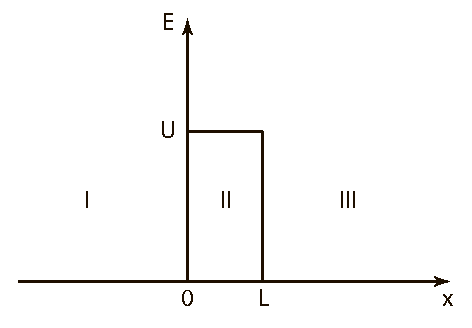
\includegraphics[width=0.5\textwidth]{images/wall}
\end{wrapfigure}

Разобъём пространство на три области. Первая -- до барьера, вторая 
барьер и третья после барьера. Тогда уравнение Шрёдингера для 
области \( I \) имеет вид:
\[
	-\frac{\hbar^2}{2m}\dder{\psi(x)}{x} = E\psi
\]
\[
	\dder{\psi}{x} + k^2 \psi = 0
\]

где \( k^2 = \cfrac{2mE}{\hbar^2} \).

Представим решение в виде \( \psi = e^{\lambda x} \). Подставляя в уравнение 
получаем:
\[ 
	\lambda^2 e^{\lambda x} + k^2 e^{\lambda x} = 0 \quad\Rightarrow\quad
	\lambda^2 + k^2 = 0 \quad\Rightarrow\quad \lambda = \pm ik 
\]

Тогда вид \( \psi(x) \) в области \( I \) имеет вид:
\[
	\psi_{I}(x) = A_1 e^{ikx} + B_1 e^{-ikx}
\]

Рассмотрим уравнение Шрёдингера в области \( II \):
\[
	\dder{\psi}{x} = \left( E - U(x) \right)\psi
\]

Представим решение в виде \( \psi = A_2 e^{\beta x} + B_2 e^{-\beta x} \), 
тогда уравнение:
\[
	\frac{\hbar^2 \beta^2}{2m}\psi(x) + \left( E - U(x) \right)\psi(x) = 0
\]

и коэффициент \( \beta^2 = \cfrac{2m\left( U(x) - E\right)}{\hbar^2} \). 
Тогда функция 
\[
	\psi_{II}(x) = A_2 e^{\beta x} + B_2 e^{-\beta x}
\]

имеет место при значении коэффициента \( \beta \) указанного выше.

Вид волновой функции для третьего участка будет иметь вид:
\[
	\psi_{III} = A_3 e^{ikx}
\]

то есть сохраняется член отвечающий за волну бегущую вдоль
положительного направления \( x \).

Зададим начальные условия для непрерывности волновой функции:
\[
	\left\{ \begin{array}{ll}
		\psi_{I}(0) = \psi_{II}(0) \\
		\psi_{II}(l) = \psi_{III}(l)
	\end{array} \right. \quad
	\left\{ \begin{array}{ll}
		\psi'_{I}(0) = \psi'_{II}(0) \\
		\psi'_{II}(l) = \psi'_{III}(l)
	\end{array} \right.
\]

Подставляя уравнения получим:
\[
	\left\{ \begin{array}{ll}
		A_1 + B_1 = A_2 + B_2 \\
		A_2 e^{\beta l} + B_2 e^{-\beta l} = A_3 e^{ikl} \\
		\left( A_1 - B_1 \right) \cdot ik = 
			\left( A_2 - B_2 \right) \cdot \beta \\
		\left( A_2 e^{\beta l} - B_2 e^{-\beta l} \right) \cdot \beta = 
			A_3 ik e^{ikl}
	\end{array} \right. \quad
	\left\{ \begin{array}{ll}
		1 + b_1 = a_2 + b_2 \\
		a_2 e^{\beta l} + b_2 e^{-\beta l} = a_3 e^{ikl} \\
		\left( 1 - b_1 \right) \cdot ik = 
			\left( a_2 - b_2 \right) \cdot \beta \\
		\left( a_2 e^{\beta l} - b_2 e^{-\beta l} \right) \cdot \beta = 
			a_3 ik e^{ikl}
	\end{array} \right.
\]

где 
\( 
	a_2 = \cfrac{A_2}{A_1}, b_1 = \cfrac{B_1}{A_1}, b_2 = \cfrac{B_2}{A_1}, 
	a_3 = \cfrac{A_3}{A_1}
\). \\

Решая систему уравнений находим:
\[
	a_2 = \frac{2n}{n+1+(n-1)\cfrac{\beta}{ik}};\quad
	b_1 = \frac{2\beta}{ik(n+1)+(n-1)\beta}
\]
\[
	b_2 = \frac{2}{n+1+(n-1)\cfrac{\beta}{ik}};\quad
	a_3 = e^{-ikl}\left( \frac{2ne^{\beta l} + 2e^{-\beta l}}
		{n+1+(n-1)\cfrac{\beta}{ik}}\right);\quad
	n = \left( \frac{ik+1}{ik-1}\right)e^{-2\beta l}
\]

Коэффициент отражения и прозрачности будут определятся равенствами:
\[
	R = \vert b_1 \vert ^2;\quad
	D = \vert a_3 \vert ^2
\]

\pagebreak
%-------------------------------------------------------------------------------

\emph{Задача №4:} Доказать эрмитовость следующих операторов: 
а) \( \hat{p}_x \);
б) \( x\hat{p}_x \);
в) \( \hat{p}^2_x \);
д) \( \hat{H} \);
Иметь в виду, что на бесконечности волновые функции и их производные обращаются 
в ноль.

\emph{Решение:}

\emph{Пункт а:}
\[
\begin{array}{ll}
	\hat{p}_x = \int\limits_{-\infty}^{+\infty} \psi_{1}^{*} \psi_2 dx =
		\int\limits_{-\infty}^{+\infty} \psi_{1}^{*} 
		\left( -i\hbar\cfrac{\partial\psi_2}{\partial x} \right) dx = 
		\Big[ u = \psi_{1}^{*}, v = \psi_{2} \Big] = \\ =
		\left( \psi_{1}^{*}\psi_{2} \Big\vert_{-\infty}^{+\infty} -
		\int\limits_{-\infty}^{+\infty} \psi_{2} 
		\left[ i\hbar \cfrac{\partial\psi_{1}^{*}}{\partial x} \right] dx \right) =
		\int\limits_{-\infty}^{+\infty} \psi_{2} 
		\left[ -i\hbar \cfrac{\partial\psi_{1}^{*}}{\partial x} \right] dx =
		\int\limits_{-\infty}^{+\infty} \psi_{2} \hat{p}_x \psi_{1}^{*}
\end{array}
\]

\emph{Пункт б:}
\[
\begin{array}{ll}
	x\hat{p}_{x} = \int\limits_{-\infty}^{+\infty} \psi_{1}^{*} x\hat{p}_{x}
		\psi_{2} dx = -i\hbar \int\limits_{-\infty}^{+\infty} \psi_{1}^{*}
		x\cfrac{\partial\psi_2}{\partial x} dx =
		\Big[ u = -i\hbar\psi_{1}^{*}, v = \psi_{2} \Big] = \\ =
		-i\hbar\left( \psi_{1}^{*} x \psi_{2} 
		\Big\vert_{-\infty}^{+\infty} - 
		\int\limits_{-\infty}^{+\infty} \psi_{2} 
		\cfrac{\partial \psi_{1}^{*} x}{\partial x} dx \right) =
		i\hbar\int\limits_{-\infty}^{+\infty} \psi_{2} 
		\left( x\cfrac{\partial\psi_{1}^{*}}{\partial x} + \psi_{1}^{*} \right) =
		i\hbar\int\limits_{-\infty}^{+\infty} \psi_{2} 
		\hat{p}_x \left( \psi_{1}^{*} x \right)
\end{array}
\]

\emph{Пункт в:}
\[
\begin{array}{ll}
	\hat{p}^2_x = \int\limits_{-\infty}^{+\infty} \psi_{1}^{*} \Big( \hat{p}_{x} 
		\hat{p}_{x} \psi_{2} \Big) = 
		\int\limits_{-\infty}^{+\infty} \psi_{1}^{*} \left( 
		-\hbar^{2} \cfrac{\partial^{2} \psi_{2}}{\partial x^2} \right) =
		\Big[ u = -\hbar^2 \psi_{1}^{*}, 
		v = \cfrac{\partial \psi_{2}}{\partial x} \Big] = \\
		-\hbar^{2} \psi_{1}^{*} \cfrac{\partial^{2} \psi_{2}}{\partial x^2} 
		\Big\vert_{-\infty}^{+\infty} + \hbar^{2} \int\limits_{-\infty}^{+\infty}
		\cfrac{\partial\psi_{2}}{\partial x}
		\cfrac{\partial\psi_{1}^{*}}{\partial x} dx =
		\hbar^{2}\left( 
		\cfrac{\partial\psi_{1}^{*}}{\partial x} \psi_{2}\right)
		\Big\vert_{-\infty}^{+\infty} -\hbar^{2} \int\limits_{-\infty}^{+\infty} 
		\psi_{2} \cfrac{\partial^{2}\psi_{1}^{*}}{\partial x^2} dx = \\
		\int\limits_{-\infty}^{+\infty} \psi_{2} 
		\left( -\hbar^{2} \cfrac{\partial^{2}\psi_{1}^{*}}{\partial x^2} \right)dx =
		\int\limits_{-\infty}^{+\infty} \psi_{2} 
		\Big( \hat{p}_{x} \hat{p}_{x} \psi_{1}^{*} \Big) dx 
\end{array}
\]

Отталкиваясь от пункта \emph{в}, можно интерполировать решение пункта \emph{д} по 
трём координатам, так как \( \hat{H} \) можно выразить в виде:
\[
	\hat{H} = \hat{T} + \hat{U} = \Big[ \text{ при условии } U = 0 \Big] = 
	-\frac{\hbar^2}{2m}\nabla^{2} = -\frac{\hbar^2}{2m}\left( 
	\frac{\partial^2}{\partial x^2} + \frac{\partial^2}{\partial y^2} + 
	\frac{\partial^2}{\partial z^2}\right)
\]
\[
\begin{array}{ll}
	\int \psi^{*} \hat{C} \psi = \int \psi^{*} \Big( A \pm B \Big) \psi = 
	\int \psi^{*} \hat{A} \psi \pm \int \psi^{*} \hat{B} \psi = 
	\int \psi \hat{A}^{*} \psi^{*} \pm \int \psi \hat{B}^{*} \psi^{*} = \\ =
	\int \psi \Big( \hat{A}^{*} \pm \hat{B}^{*} \Big) \psi^{*} = 
	\int \psi \Big( \hat{A} \pm \hat{B} \Big)^{*} \psi^{*} = 
	\int \psi \hat{C}^{*} \psi^{*}
\end{array}
\]

С учётом выражения выше, действуя аналогично пункту \emph{в} можно доказать 
эрмитовость \( \hat{H} \).

\pagebreak
%-------------------------------------------------------------------------------

\emph{Задача №5:} Найти собственное значение оператора и собственные функции 
оператора \( \hat{A} = \cfrac{1}{x^n}\cfrac{d}{dx} \).

\emph{Решение:}

Найдём собственную функцию оператора \( \hat{A} \):
\[
	\hat{A}\psi(x) = A\psi(x); \quad
	\cfrac{1}{x^n}\cfrac{d\psi}{dx} = A\psi; \quad
	\cfrac{d\psi}{dx} = A x^n \psi
\]
\[
	\cfrac{d\psi}{\psi} = A x^n dx \quad \Rightarrow \quad
	\psi = C_1 exp\left[ A \frac{x^{n+1}}{n+1} \right]
\]

%-------------------------------------------------------------------------------

\end{document}
